\section{Software empleado en el proyecto}
\subsection{ROS}
ROS (Robotic Operating System) consite en un framework para la robótica sobre el que desarrolladores de cualquier 
ambito pueden aportar soluciones modulares a los sistemas de forma general. La modularidad de ROS hace que desarrollar 
un nuevo sistema o prototipo pueda ser una tarea tan sencilla como interconectar módulos de otros desarrolladores con 
los propios.\\
Esta característica lo hace idoneo para un proyecto como este en el que el uso de técnicas de percepción, 
mapeado, localization, etc, complejas se escapa del alcance; y solo sea necesario el desarrollo de modulos específicos de este robot
que sean capaces de comunicarse con aquellos más complejos y sean capaces de proporcionarle los datos necesarios para implementar los
algoritmos de SLAM.
\subsubsection{Computación distribuida con ROS-Multimaster Package}
Las técnicas de SLAM a testear en el robot desarrollado son computacionalmente costosas. De manera genérica a los metodos de SLAM visual usados, 
para cada frame capturado por la camara el algoritmo extrae `features' de la imagen, las alamacena y compara los conjuntos con los de otro frame. 
Entre ambos frames el algoritmo calcula una matriz de transformación homogenea con la cual se es capaz de saber, al menos localmente, cuanto y como se ha
desplazado el robot. Sumado a eso cada algoritmo tiene su forma propia de localizar globalmente en el mapa creado al robot. Todo este coste computacional es
imposible asumirlo desde una Raspberry-Pi, por lo que surge la necesidad de hacer el procesado en un servidor remoto al robot en tiempo real con las 
dificultades que eso conlleva, entre ellas y la mas importante, la sincronización de datos.\\
Bajo estas condiciones de diseño y restricciones aparece una solución de la comunidad: ROS multimaster\_fkie. La premisa que lo rige es simple, dado un sistema mutirobot
cada elemento mantiene la ejecución de 2 nodos locales, \textit{master\_discovery} y \textit{master\_sync}; el primero es el encargado de mantener una lista del resto 
de \textit{roscores} disponibles en la red y de publicar el suyo propio como activo. El otro es el encargado de suscribir su \textit{core} los nodos de otros \textit{cores}.\\
Des esta forma todos tienen acceso de una forma hasta cierto punto `real-time' a los recursos del resto. 
\begin{figure}[!ht]
    \centering
    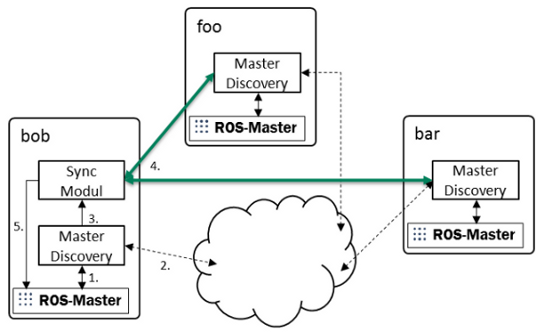
\includegraphics[width=0.6\textwidth]{images/ros_multimaster.png}
    \caption{Esquema del funncionamiento básico del paquete Multimaster}
\end{figure}\\
En este proyecto su integración se ha llevado a cabo lanzando en la Raspberry-Pi y en otro PC los nodos correspondientes siendo la Raspberry-Pi la 
suministradora de información y el PC el encargado de procesarla.
\subsubsection{Interfaz con IMU}
Como ya se ha visto en la seccion \ref{imu_hardw}, al robot se le ha dotado con una IMU de 9 grados de libertad a fin de obtener medidas de aceleraciones.\\
La conexión se hace a través de una linea por protocolo $I^2C$, por lo que ha sido necesario el desarrollo de 2 `wrapers' en Python de funciones de bajo nivel; uno para el acceso a las
funciones de comunicación $I^2C$ a nivel de registros hardware y otro a nivel de funciones elementales para el manejo de los datos de la IMU.\\
Sobre ambos `wrapers' se ha escrito el nodo de ROS encargado de publicar los datos en 2 `topics', \textit{imu1\_rawImu} y \textit{imu1\_scaImu}, con los datos tal y como llegan 
de la IMU en el primero y reescalados en el segundo. El tipo de mensaje en el que se publican los datos es de tipo \textit{\href{http://docs.ros.org/melodic/api/sensor_msgs/html/msg/Imu.html}{sensor\_msgs/Imu}}.\\
Como se trata de un sensor de bajo nivel que aporta información a los estratos más bajos del control, para poder disponer depués de mayor ancho de banda, se ha elegido una frecuencia de muestreo del sensor de $50\ [Hz]$; sufucientemente alta para no comprometer la estabildiad del sistema
 pero tambien lo sufucientemente baja como para no saturar el ordenador de abordo (teniendo en cuenta que este también deberá mantener un flujo constante de imagenes capturadas por la cámara, con el coste que eso conlleva).
\subsubsection{Interfaz con encoders}\label{enc_soft}
Otro sensor añadido son los encoders mencionados en \ref{enc_hard}. Para su programación se ha desarrollado un `wraper' en C++ de la librería para Raspberr-Pi 3B \textit{pigpio} 
\cite{pigpio}. Como los encoders solo pueden ofrecer información de la magnitud de la velocidad y no del sentido es necesario hacer una conversión a nivel de sofware para poder
tener esa información.\\
Esto se hace suscribiendo el nodo creado al `topic' \textit{cmd\_vel}, de forma que de ahí se obtiene la referencia del sentido en el que se mueve el robot. Esta referencia se usa para reajustar el signo de las velocidades 
leidas directamente de los 6 encoders y publicarlas en el topic \textit{encoders} con el tipo de mensaje \textit{\href{http://docs.ros.org/jade/api/std_msgs/html/msg/Float64MultiArray.html}{std\_msgs/Float64MultiArray}}. La medida de los encoders, al tratarse de medidas de baja calidad con valores dispersos, han sido necesaria filtrarlas también.\\
En cuanto a la frecuencia de muestreo, se ha seguido la misma filosofia que con la programación del nodo de la IMU y se ha decido muestear a $50\ [Hz]$.
\subsubsection{Odometría}
Como se dispone de una medida de la velocidad de las ruedas se consideró tanto interesante como oportuno el desarrollo de un nodo en ROS en el que se calculase la odometría con los encoders.
Para ello se han hecho una serie de suposiciones y simplificaciones del modelo del robot que después, en base a los resultados obtenidos, se han demostrado bastante acertadas.\\
La primera es que las ruedas tienen un modelo de rodadura perfecto y no deslizan en el suelo. Esto no es cierto en realidad y supone una fuente de errores importantes por la deriva que acumulan las posiciones estimadas, errores que son corregidos mediante una fusión sensorial.\\
Otra simplicación hecha es que el modelo del robot consiste en un modelo diferencial de 2 ruedas. En base a esto a cada rueda `virtual' se le asigna el promedio de la velocidad de las 3 ruedas de cada bancada, cosa que simplifica mucho los cálculos.\\

Este nodo se suscribe al desarrollado en \ref{enc_soft} en el `topic' \textit{encoders}, y cada vez que llega un mensaje nuevo con los datos de los 
encoders calcula el avance del robot en base al modelo propuesto. La publicación de los datos se hace en el `topic' \textit{odom} a un ratio de $25\ [Hz]$ 
con un mensaje del tipo \textit{\href{http://docs.ros.org/melodic/api/nav_msgs/html/msg/Odometry.html}{nav\_msgs/Odometry}}.

\subsubsection{Interfaz Raspberry-Pi/Arduino}
La comunicación por puerto serie se implementa haciendo uso de la librería \textit{CmdMessenger}. MIGUEL LAS PUTAS REFERENCIAS ACUÉRDATE., que permite definir comandos (con la posibilidad de asociarles argumentos y callbacks) de forma eficiente y sencilla.
Por la parte de la Raspberry, se usan las librerías CmdMessenger (escrita en c) o su alternativa PyCmdMessenger (en Python) en el nodo serial\_com.py para transmitir por el puerto serie.\\
Los siguientes comandos son los más importantes \\
Cmd\_off; Al recibir este comando el micro pasa a no hacer nada, comportándose como un apagado de emergencia. \par
De esta forma es sencillo publicar un tópico de 'comandos del sistema', como apagar o funciones de debugeo, y otros tópicos para los datos que hayan de retransmitirse. Cuando llegan datos desde el arduino, se ejecuta un callback (de la librería externa, no de ROS) que publica dicha información el tópico correspondiente. Si es el caso contrario, y se busca enviar datos al arduino, el nodo se subscribirá al tópico con ese dato y en el callback asociado (ahora sí de ROS) se envía al arduino.

\subsubsection{Interfaz Arduino/Motores}
Same old same old
\subsection{Implementación de filtro estadístico}
La información que el sistema obtiene de los sensores está sujeta a ruido e incertidumbres de la medida. A fin de minimizar los errores y mejorar la estimación de la posicion y velocidad del robot se ha 
considerado que era de especial interes y utilidad la aplicación de un filtro recursivo Bayesiano como estimador de estados, en concreto el filtro de Kalman extendido.
\subsubsection{ROS-Robot Localization Package}

\subsection{Arquitectura general del sistema}
\begin{figure}[!ht]
    \centering
    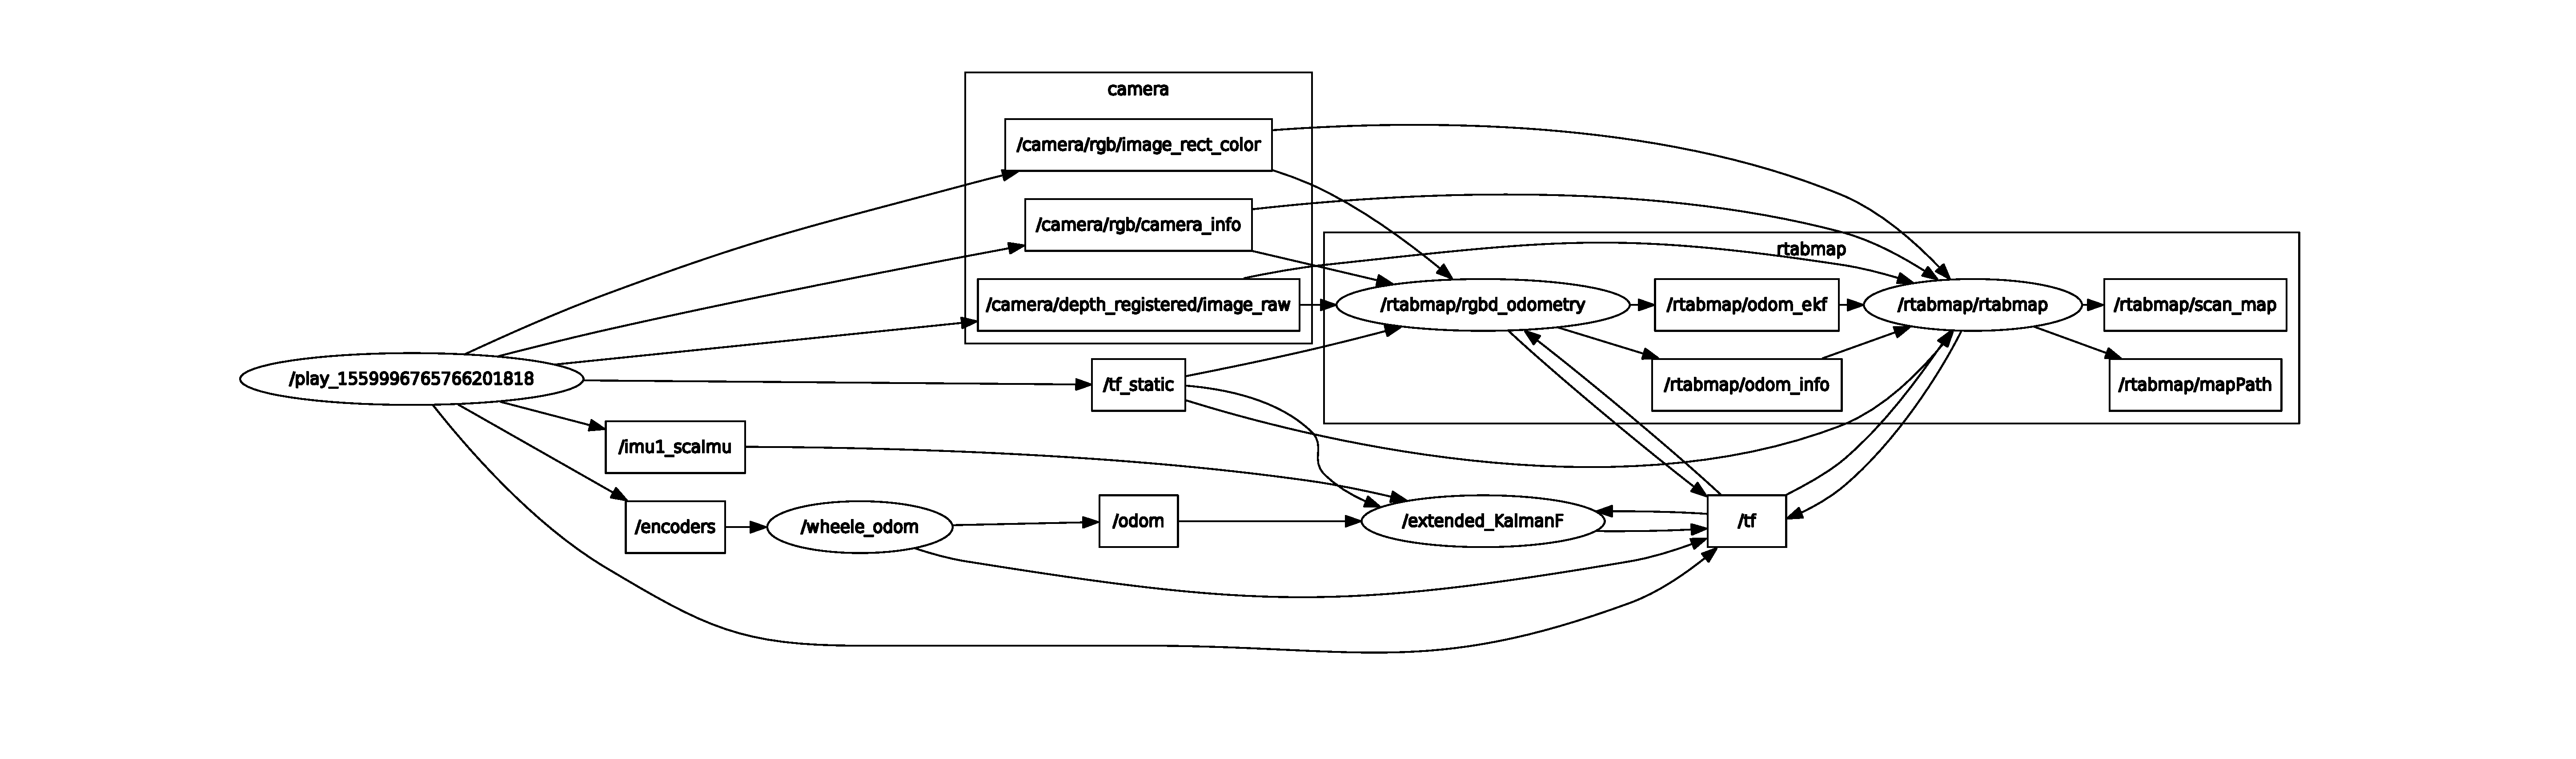
\includegraphics[width=\textwidth]{images/rqt_graphs/graph_RTABMAP.pdf}
    \caption{Captura de los nodos ejecutandose durante uno de los experimentos realizados con el robot}
    \label{rqt01}
\end{figure}
